\documentclass[conference]{IEEEtran}
\usepackage{graphicx,amsmath,array,booktabs,url,balance}
\usepackage[hidelinks]{hyperref}
\begin{document}
\title{Comparative Evaluation of Machine Learning and Deep Learning for Synthetic Financial Fraud Detection}
\author{\IEEEauthorblockN{Animesh B. Labh}
\IEEEauthorblockA{School of Computer Science\\and Engineering\\Vellore Institute of Technology\\Vellore, India\\Registration No.: 23BCE0415}\and\IEEEauthorblockN{Kushagra Dhelia}
\IEEEauthorblockA{School of Computer Science\\and Engineering\\Vellore Institute of Technology\\Vellore, India\\Registration No.: 23BDS0091}\and\IEEEauthorblockN{Dhruv Singh}
\IEEEauthorblockA{School of Computer Science\\and Engineering\\Vellore Institute of Technology\\Vellore, India\\Registration No.: 23BCE0374}}
\maketitle
\begin{abstract}
Financial fraud detection requires a useful balance between missed fraud and unnecessary alerts. This study compares random forest, extreme gradient boosting, a multilayer neural classifier, and an autoencoder within a reproducible transaction review prototype. The experiment uses 15,000 locally generated synthetic transactions, including 225 fraudulent records. A stratified 60/20/20 split separates training, validation, and testing. Imputation and shared scaling are fitted on training records; categorical minority oversampling is restricted to supervised training. The autoencoder learns reconstruction from legitimate training records. Each decision threshold maximizes validation F1, while model selection uses validation average precision. Extreme gradient boosting achieves the highest validation average precision, 0.9020, and remains the selected model. On 3,000 test transactions containing 45 fraud cases, the autoencoder attains an F1 score of 0.9425 and average precision of 0.9586. The neural classifier identifies 40 fraud cases without false positives; random forest identifies 42 with nine false positives. These results describe different operating tradeoffs on one synthetic benchmark. Feature attribution and a Kafka-compatible ingestion prototype support transaction review, while synthetic data construction, closing-balance inputs, and a single experimental split limit conclusions about real financial deployment.
\end{abstract}
\begin{IEEEkeywords}
financial fraud detection, imbalanced classification, synthetic transactions, autoencoder, model explainability
\end{IEEEkeywords}
\section{Introduction}
Fraud screening is a classification problem with an uneven error burden. A missed fraudulent transaction can cause financial loss, while an incorrect alert consumes review effort and can interrupt a legitimate payment. When fraud is rare, a high accuracy value can coexist with poor detection. This makes the operating threshold and the number of alerts as relevant as the choice of model.

Access to representative financial records is constrained by confidentiality and data ownership. Simulation provides a practical setting for implementing and inspecting fraud detection workflows. PaySim is an established example of synthetic mobile-money simulation \cite{r1}. The present study uses an independent local generator with a similar transaction schema; it does not use the official PaySim dataset or real bank records.

The research question is whether tree ensembles, a neural classifier, and reconstruction-based anomaly detection produce different useful operating points when they share a fixed transaction representation and untouched validation and test prevalence. Precision-recall analysis receives particular attention because it describes positive predictions under class imbalance \cite{r2}. We also examine whether the model preferred during validation remains the strongest model under each test metric.

The study contributes a documented four-model comparison, a training-only preprocessing and sampling procedure, and an inspection interface that connects model outputs with balance arithmetic and event ingestion. Its contribution is an evaluated prototype and an account of the resulting tradeoffs. The experiment does not introduce a new learning algorithm or establish performance on a financial institution's transaction stream.

\section{Related work}
Random forests combine randomized decision trees and provide a baseline for nonlinear tabular classification \cite{r3}. Extreme gradient boosting, implemented by XGBoost, fits an additive tree ensemble with a regularized learning objective \cite{r4}. These approaches can represent interactions between amounts, transaction categories, and account balances without requiring a manually specified decision boundary.

A multilayer perceptron learns a discriminative boundary from labeled examples. An autoencoder instead maps an input through a lower-dimensional representation and attempts to reconstruct it. Reconstruction error can identify observations that differ from the training distribution. Zhou and Paffenroth study a robust deep autoencoder that separates noise and anomalous components \cite{r5}. Our implementation uses a conventional reconstruction network trained on legitimate examples and does not implement their robust decomposition.

Synthetic Minority Over-sampling Technique (SMOTE) creates minority examples by interpolation \cite{r6}. The imbalanced-learn toolbox provides compatible sampling implementations \cite{r7}. For data containing numerical and categorical attributes, SMOTE for nominal and continuous features (SMOTE-NC) handles category selection separately from numeric interpolation \cite{r8}. This distinction matters here because fractional transaction categories would have no valid operational meaning.

SHapley Additive exPlanations (SHAP) assigns additive feature contributions to model predictions \cite{r9}. Such explanations help inspect a detector's dependence on its inputs, but they do not establish the cause of fraud. Apache Kafka provides partitioned event logs and consumer groups for event processing \cite{r10}. We use these ideas to organize ingestion and alert records; classifier evaluation and distributed-system validation remain separate tasks.

\section{Dataset and feature preparation}
\subsection{Synthetic transaction construction}
The benchmark contains 15,000 records: 14,775 legitimate and 225 fraudulent transactions. Fraud prevalence is 1.5\%, corresponding to a legitimate-to-fraud ratio of 65.67:1. Records contain a transaction step, one of five transaction types, an amount, opening and closing origin balances, opening and closing destination balances, a fraud label, and a rule-generated flag. The step is an independently sampled integer from 1 to 743, without a documented physical time unit or account history.

The generator uses different distributions for the two classes. Legitimate origin balance changes approximate the transaction amount with Gaussian noise. Fraudulent origin debits use 65-100\% of the amount, while fraudulent destination opening balances are sampled from four fixed values. Some fraudulent destinations have a zero closing balance. These rules create an inspectable benchmark, but also make balance discrepancies informative by construction. High performance can therefore reflect recovery of generator rules.

\subsection{Partitions and input schema}
Table I gives the stratified random partitions, all generated with seed 42. Duplicate labeled input rows are removed before partitioning; the current dataset contains no duplicates or missing cells. The saved partition indices are disjoint. The fraud label is the prediction target, and the rule-generated flag is excluded from model inputs.

\begin{table}[t]
\caption{Original data partitions}
\centering\footnotesize
\setlength{\tabcolsep}{3pt}
\begin{tabular}{lrrr}
\toprule
Partition & Legitimate & Fraud & Total\\
\midrule
Training & 8,865 & 135 & 9,000\\
Validation & 2,955 & 45 & 3,000\\
Test & 2,955 & 45 & 3,000\\
All records & 14,775 & 225 & 15,000\\
\bottomrule
\end{tabular}
\end{table}
Numeric imputation uses medians from the training partition; a missing transaction type uses the training mode. These operations are retained for inference even though this benchmark is complete. A fixed schema prevents a new batch from changing feature order or category columns. Six numeric raw inputs and five type indicators are combined with three engineered quantities to obtain 14 model inputs.

\subsection{Balance features and scaling}
Let a denote the amount, and let b\_o and b\_d denote origin and destination balances, with superscripts old and new. The two discrepancy features are defined as

\begin{equation}
\Delta_o=b_o^{\mathrm{new}}+a-b_o^{\mathrm{old}}
\end{equation}
\begin{equation}
\Delta_d=b_d^{\mathrm{old}}+a-b_d^{\mathrm{new}}.
\end{equation}
The amount-to-opening-origin-balance ratio is a/(b\_o(old) + 0.00001) when the opening balance is positive, and zero otherwise. The shared RobustScaler centers each feature by its training median and scales it by its training interquartile range. Neither validation nor test rows fit this transformation.

Closing balances describe a completed transaction. Consequently, these features support retrospective review, including review immediately after event ingestion. They cannot be assumed available before a payment is authorized. A discrepancy also depends on ledger conventions and transaction type; it is an input observation rather than proof of fraud.

\subsection{Training-only imbalance handling}
SMOTE-NC is applied only to the supervised training partition. The five type indicators are temporarily decoded to one categorical attribute, sampled with five minority neighbors and seed 42, and re-encoded. Numeric features are interpolated in the shared scaled space. Sampling to a 1:1 ratio produces 8,865 examples per class, or 17,730 supervised training examples. Validation and test records retain the original 1.5\% fraud prevalence.

The autoencoder receives the original 8,865 legitimate training examples instead of oversampled data. Its internal standardization and network updates use those legitimate examples. The shared RobustScaler has already been fitted on all 9,000 training examples, so the entire preprocessing path is not exclusively fitted on legitimate data. Fig. 1 summarizes the training and evaluation boundaries.

\begin{figure}[t]
\centering
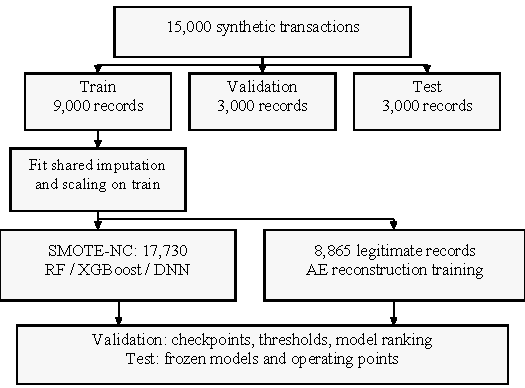
\includegraphics[width=\columnwidth]{images/pipeline.pdf}
\caption{Partitioning and model fitting. All learned preprocessing excludes validation and test records; thresholds use validation only.}
\label{fig:pipeline}
\end{figure}
\section{Models and validation protocol}
\subsection{Tree ensembles and neural classifier}
Random forest uses 150 trees, maximum depth 12, and balanced\_subsample class weights. XGBoost uses 150 estimators, maximum depth 6, learning rate 0.08, and log-loss evaluation. Both use seed 42 and two workers. These are fixed configurations in this experiment; there is no reported hyperparameter search.

The deep neural network (DNN) is an MLPClassifier with a 14-64-32-16-1 architecture, rectified linear hidden activations, and a binary output. Adam uses a learning rate of 0.001, L2 coefficient 0.001, and batch size 256. An internal StandardScaler is fitted on the balanced training data, followed by clipping to [-12, 12]. Validation average precision determines the saved checkpoint, with a 120-epoch limit and patience of 15. The saved network contains 3,585 parameters and restores epoch 33 after 48 epochs of training.

\subsection{Autoencoder and anomaly score}
The autoencoder (AE) is an MLPRegressor with architecture 14-64-32-8-32-64-14, rectified linear hidden activations, and a linear reconstruction output. It uses Adam, learning rate 0.001, L2 coefficient 0.001, batch size 256, a 100-epoch limit, and patience of 12. Legitimate training inputs fit its internal StandardScaler; transformed values are clipped to [-20, 20]. Checkpoint selection minimizes reconstruction mean squared error on legitimate validation examples. The saved model has 6,614 parameters and restores epoch 99 after 100 epochs.

For transformed input z, let f(z) denote the network reconstruction. The mean squared reconstruction error and normalized score are

\begin{equation}
e(x)=\frac{1}{14}\sum_{j=1}^{14}(z_j-f_j(z))^2
\end{equation}
\begin{equation}
s_{\mathrm{AE}}(x)=\frac{e(x)}{e(x)+q_{0.99}}.
\end{equation}
Here q\_0.99 is the 99th percentile of legitimate training reconstruction errors, lower-bounded by 10\textasciicircum{}(-12). The score is bounded and increases with reconstruction error. It is not a calibrated fraud probability. Supervised classifier scores are also treated as uncalibrated because resampling changes the training class prior and no calibration experiment is performed.

\subsection{Thresholds and model selection}
For each model m, a transaction is flagged when its score reaches threshold tau\_m. Threshold selection considers every distinct observed validation score. The selected threshold maximizes validation F1; ties use the higher threshold. The F1 definition is

\begin{equation}
F_1=\frac{2TP}{2TP+FP+FN}.
\end{equation}
Model ranking is separate from threshold selection. The primary ranking metric is validation average precision (AP), with validation F1 and recall as tie-breakers. AP is the sum of precision weighted by successive recall increments. The project files label this quantity PR-AUC, but the implementation uses average\_precision\_score, not a trapezoidal precision-recall integral. We use AP throughout this paper.

Table II reports validation performance and the resulting thresholds. XGBoost has the highest validation AP, 0.9020, and is retained as the selected model. The AE has the highest validation F1, 0.8889. Their different rankings follow from the stated selection objectives. All thresholds are fixed before evaluating the test partition.

\begin{table}[t]
\caption{Validation selection and operating points}
\centering\footnotesize
\setlength{\tabcolsep}{3pt}
\begin{tabular}{lrrrr}
\toprule
Model & Threshold & AP & F1 & Recall\\
\midrule
RF & 0.740000 & 0.8879 & 0.8434 & 0.7778\\
XGBoost & 0.944544 & 0.9020 & 0.8706 & 0.8222\\
DNN & 0.999329 & 0.8473 & 0.8608 & 0.7556\\
AE & 0.870672 & 0.8828 & 0.8889 & 0.8000\\
\bottomrule
\end{tabular}
\end{table}
The DNN threshold near one reflects this model's score distribution, not near-certain fraud risk. Neural checkpoint selection, threshold tuning, and model ranking reuse the same validation partition. This can produce selection optimism, although the test records do not participate in those decisions.

\section{Experimental results}
\subsection{Classification and ranking performance}
Tables III and IV report the test results using the frozen validation thresholds. The test partition contains 2,955 legitimate transactions and 45 fraud cases. A classifier that always predicts legitimate would achieve 98.5\% accuracy with zero fraud recall. Observed accuracy is 99.60\% for RF, 99.67\% for XGBoost, and 99.83\% for both neural models. The error counts provide a more useful comparison than those accuracy values alone.

\begin{table}[t]
\caption{Performance on the held-out test partition}
\centering\footnotesize
\setlength{\tabcolsep}{3pt}
\begin{tabular}{lrrrr}
\toprule
Model & Precision & Recall & F1 & AP\\
\midrule
RF & 0.8235 & 0.9333 & 0.8750 & 0.9581\\
XGBoost & 0.8889 & 0.8889 & 0.8889 & 0.9418\\
DNN & 1.0000 & 0.8889 & 0.9412 & 0.9307\\
AE & 0.9762 & 0.9111 & 0.9425 & 0.9586\\
\bottomrule
\end{tabular}
\end{table}
\begin{table}[t]
\caption{Test confusion counts and ROC area}
\centering\footnotesize
\setlength{\tabcolsep}{3pt}
\begin{tabular}{lrrrrr}
\toprule
Model & TP & FP & TN & FN & ROC area\\
\midrule
RF & 42 & 9 & 2,946 & 3 & 0.9989\\
XGBoost & 40 & 5 & 2,950 & 5 & 0.9968\\
DNN & 40 & 0 & 2,955 & 5 & 0.9863\\
AE & 41 & 1 & 2,954 & 4 & 0.9909\\
\bottomrule
\end{tabular}
\end{table}
RF has the highest recall, identifying 42 of 45 fraud cases, but produces nine false alerts. XGBoost identifies 40 fraud cases and produces five false alerts. The DNN identifies the same number of fraud cases with no false positives in this test partition. AE identifies 41 fraud cases with one false positive, giving the highest observed F1, 0.9425. Specificity ranges from 0.9970 for RF to 1.0000 for DNN.

The area under the receiver operating characteristic curve (ROC area) is highest for RF, 0.9989, while test AP is highest for AE, 0.9586. Fig. 2 plots test precision-recall curves from the saved transaction scores. These curves describe ranking performance across thresholds; the confusion counts describe one selected operating point. A model can rank strongly yet produce more false alerts at its chosen threshold.

\begin{figure}[t]
\centering
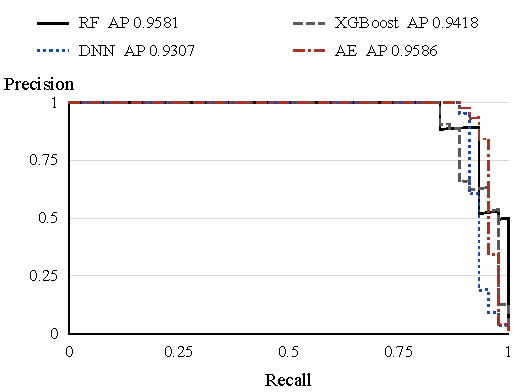
\includegraphics[width=\columnwidth]{images/precision_recall.pdf}
\caption{Test precision-recall curves computed from saved scores. AP denotes average precision; each curve uses the same 45 fraud cases.}
\label{fig:precision_recall}
\end{figure}
\subsection{Interpreting the observed differences}
The AE-DNN F1 difference is approximately 0.00135. In count terms, AE detects one additional fraud case and raises one additional false alert. AE also exceeds RF AP by only about 0.00052. These narrow differences do not establish statistical superiority. With 45 fraud cases, one additional detection changes recall by 1/45, or 2.22 percentage points.

Validation and test rankings differ. XGBoost has the best validation AP, while AE and RF have higher test AP. The selected model is therefore kept as XGBoost rather than being replaced after test inspection. This preserves the original selection protocol. Repeated partitions or an independent dataset would be needed to assess whether any ranking is stable.

The results support choosing an operating point according to review capacity and missed-fraud costs. RF supplies the highest observed recall; DNN supplies the fewest observed false alerts. There is no cost-based utility study here, so the experiment cannot identify an economically optimal policy. Likewise, the absence of an oversampling ablation prevents attributing any improvement specifically to SMOTE-NC.

\section{Explainability and review system}
\subsection{Feature attribution and balance inspection}
Tree SHAP is applied to the selected XGBoost model on a random sample of up to 500 test records with seed 42. The saved mean absolute attribution plot ranks origin balance discrepancy first, destination opening balance second, and destination balance discrepancy third. This ranking is consistent with the generator's class-dependent balance rules. No numeric contribution percentage is claimed because the experiment does not retain a numeric attribution summary.

The interface also displays arithmetic balance discrepancies, account depletion observations, model-specific scores, and the thresholds used for decisions. These observations help a reviewer inspect a completed transaction. They do not independently verify fraud, infer intent, or establish a regulatory explanation requirement. Risk categories displayed by the prototype are advisory labels derived from scores.

\subsection{Batch review and event ingestion}
The review application supports single-record scoring, batch uploads, side-by-side model outputs, and retained review records. Its any-model review flag is the logical OR of the four threshold decisions. This rule is a review aid and is not a trained ensemble. Scores from different models are not averaged because they have different meanings and have not been calibrated to a common probability scale.

The event prototype serializes transactions as JSON, publishes them to financial.transactions, runs the saved preprocessing and inference components, and emits structured review alerts to financial.fraud-alerts. An in-process broker using queues and locks supports offline demonstrations and automated functional checks. A real Kafka connection is a separate execution mode. Kafka's partition ordering does not imply global ordering or automatic exactly-once behavior across inference and alert handling \cite{r10}.

The consumer records processing latency for individual events. There is no retained controlled experiment measuring throughput, tail latency, broker failure recovery, or multi-node scaling. We therefore report the streaming path as an implemented integration prototype and make no numerical latency or production-availability claim. Event arrival also does not change the retrospective nature of closing-balance features.

\section{Limitations and reproducibility}
The main validity limitation is the synthetic data generator. Amount and balance patterns are sampled according to explicit class rules, with no linked customer accounts, delayed investigator labels, changing fraud strategies, or verified real transaction behavior. Random stratification preserves class prevalence but does not evaluate temporal generalization. The models may learn generator-specific regularities that disappear on real records.

The comparison uses one seed and fixed model settings. It includes no external benchmark, repeated-run uncertainty analysis, temporal holdout, feature ablation, or probability calibration. Validation reuse may favor selected checkpoints and thresholds. Only 45 fraud cases occur in the test partition, so zero observed DNN false positives and small F1 differences should not be projected to future streams.

The autoencoder is legitimate-only at the reconstruction-training stage, while its shared preprocessing uses all training records and its fraud threshold uses labeled validation data. It is therefore not a fully label-free detector. Moreover, SMOTE-NC preserves transaction categories, but the interpolated amount-to-balance ratio generally differs from the ratio recomputed from interpolated raw balances. The experiment does not measure the effect of such combinations.

Reproduction is supported by the generator, dependency lock file, saved split indices, model metadata, thresholds, learning histories, and per-record test predictions. The dataset SHA-256 begins c0b407c3bb35167e; the complete digest is retained in experiment\_metadata.json. The recorded environment uses Python 3.12.14, NumPy 2.3.5, pandas 3.0.1, scikit-learn 1.9.1, XGBoost 3.4.1, imbalanced-learn 0.14.2, and SHAP 0.54.1. All reported metrics come from the saved experiment with seed 42.

A stronger follow-up study would compare an external financial dataset, use time-respecting partitions where account history exists, and repeat training across seeds. Removing closing-balance inputs would test whether useful performance survives a pre-authorization feature constraint. Sampling ablations, calibrated scores, and explicit review-cost models would then help choose an operating policy. Broker load and recovery experiments are required before assigning service-level targets to the event pipeline.

\section{Conclusion}
On this locally generated benchmark, the four model families produce different fraud detection tradeoffs under a common validation protocol. XGBoost is selected by validation AP of 0.9020. On the untouched test partition, AE attains F1 of 0.9425 and AP of 0.9586, RF detects the most fraud cases, and DNN produces no observed false alerts. These findings support inspecting error counts and threshold objectives alongside ranking metrics. The prototype connects these decisions with balance inspection and event ingestion, while real-data validation and broader experimental replication remain necessary to establish practical performance.

\balance
\begin{thebibliography}{10}
\bibitem{r1} E. A. Lopez-Rojas, A. Elmir, and S. Axelsson, "PaySim: A financial mobile money simulator for fraud detection," in Proc. 28th European Modeling and Simulation Symp. (EMSS), Larnaca, Cyprus, 2016, pp. 249-255. \url{https://www.msc-les.org/proceedings/emss/2016/EMSS2016_249.pdf}.
\bibitem{r2} T. Saito and M. Rehmsmeier, "The precision-recall plot is more informative than the ROC plot when evaluating binary classifiers on imbalanced datasets," PLOS ONE, vol. 10, no. 3, Art. no. e0118432, 2015, doi: 10.1371/journal.pone.0118432. \url{https://doi.org/10.1371/journal.pone.0118432}.
\bibitem{r3} L. Breiman, "Random forests," Mach. Learn., vol. 45, no. 1, pp. 5-32, 2001, doi: 10.1023/A:1010933404324. \url{https://doi.org/10.1023/A:1010933404324}.
\bibitem{r4} T. Chen and C. Guestrin, "XGBoost: A scalable tree boosting system," in Proc. 22nd ACM SIGKDD Int. Conf. Knowledge Discovery and Data Mining, 2016, pp. 785-794, doi: 10.1145/2939672.2939785. \url{https://doi.org/10.1145/2939672.2939785}.
\bibitem{r5} C. Zhou and R. C. Paffenroth, "Anomaly detection with robust deep autoencoders," in Proc. 23rd ACM SIGKDD Int. Conf. Knowledge Discovery and Data Mining, 2017, pp. 665-674, doi: 10.1145/3097983.3098052. \url{https://doi.org/10.1145/3097983.3098052}.
\bibitem{r6} N. V. Chawla, K. W. Bowyer, L. O. Hall, and W. P. Kegelmeyer, "SMOTE: Synthetic minority over-sampling technique," J. Artif. Intell. Res., vol. 16, pp. 321-357, 2002, doi: 10.1613/jair.953. \url{https://doi.org/10.1613/jair.953}.
\bibitem{r7} G. Lemaitre, F. Nogueira, and C. K. Aridas, "Imbalanced-learn: A Python toolbox to tackle the curse of imbalanced datasets in machine learning," J. Mach. Learn. Res., vol. 18, no. 17, pp. 1-5, 2017. \url{https://jmlr.org/papers/v18/16-365.html}.
\bibitem{r8} The imbalanced-learn Developers, "SMOTENC," imbalanced-learn documentation. Accessed: Oct. 19, 2026. \url{https://imbalanced-learn.org/stable/references/generated/imblearn.over_sampling.SMOTENC.html}.
\bibitem{r9} S. M. Lundberg and S.-I. Lee, "A unified approach to interpreting model predictions," in Advances in Neural Information Processing Systems, vol. 30, 2017, pp. 4765-4774. \url{https://papers.nips.cc/paper/2017/hash/8a20a8621978632d76c43dfd28b67767-Abstract.html}.
\bibitem{r10} Apache Software Foundation, "Design," Apache Kafka documentation. Accessed: Oct. 19, 2026. \url{https://kafka.apache.org/design/}.
\end{thebibliography}
\end{document}
